\chapter{Diseño e implementación}
\label{cap:diseñoeimplementación}

%Hacer intro de esta sección, supongo que cuando esté algo más hecho será más fácil hacerla.

Hemos planteado la aplicación como un modelo cliente-servidor, en la que el servidor se encargará de ejecutar el programa que lleve a cabo todos los cálculos de la ruta y se los proporcionará al cliente (dispositivo móvil) cuando este lo solicite. De esta manera, nuestro programa estará mejor organizado, será mas rápido y evitaremos que nuestro dispositivo móvil se quede sin batería rápidamente debido a una pesada carga computacional. A continuación detallaremos el diseño y los detalles técnicos de la implementación tanto del cliente como del servidor.


\section{Servidor}
El servidor constituye una parte indispensable del proyecto ya que se encarga de realizar los cálculos más pesados para no sobrecargar al dispositivo móvil. Sus principales funcionalidades son:
\begin{itemize}
	\item Almacenar la estructura e información referente al edificio mapeado.
	\item Permanecer a la escucha de cualquier cliente que solicite conexión.
	\item Solventar el posicionamiento del cliente conectado.
	\item Generar ruta óptima desde la posición actual hasta el destino indicados por el cliente.
\end{itemize} 

La aplicación servidor está diferenciada en dos partes: el código realizado en java y los archivos correspondientes al edificio que se mapea, en nuestro caso la Facultad de Informática de la UCM. Estos archivos son los xml mencionados en la Sección \ref{sec:mapeo} y un archivo json que contiene información referente a los cuadrantes que son denominados destinos en nuestra aplicación (por ejemplo, secretaría, conserjería, las aulas, la cafetería, etc). 
Buena parte del código que conforma el servidor ha sido reutilizado de trabajos anteriores, concretamente de los proyectos \textit{Generador interactivo de instrucciones de guía sobre plataformas móviles} \citep{TFGguia} y del proyecto \textit{Sistema de guía por voz en interiores} \citep{TFGMariana}. La estructura de nuestro servidor conserva la realizada en \cite{TFGguia}. Sin embargo, se han introducido cambios notorios para el desarrollo de esta aplicación que comentaremos a continuación.

\subsection{Funcionamiento del servidor}

Para entender mejor la estructura del servidor, haremos un recorrido desde la carga de la información de los archivos que representan el edificio mapeado hasta la conexión con el cliente y el cálculo de la ruta: 

\begin{itemize}
	\item \textit{Arranque del servidor:} Cuando el servidor arranca es necesario que guarde información sobre el edifico que va a mapear para que pueda dar al cliente la ruta solicitada. Esta información no es otra que la contemplada en los archivos xml de la Sección \ref{sec:mapeo}. Como ya sabemos, la estructura de estos archivos se apoya en la establecida en \cite{TFGguia}. De la misma manera, el código relacionado con la carga de estos archivos y que da lugar a las clases \textit{CargaXML} y \textit{Edificio}, está reutilizado del proyecto ya mencionado. Estas clases permiten cargar los archivos y almacenar la información referente a los cuadrantes. Para nuestro trabajo se han añadido las estructuras necesarias para guardar la información nueva incluida en los xml (como los \textit{beacons}, los metros que ocupa el cuadrante o la información adicional de este) y se han eliminado aquellas que ya no se utilizan (como coordenadas sureste y noroeste que no están presentes en nuestro proyecto). Una vez que tenemos una lista de cuadrantes, lo que se hace es generar una matriz de adyacencia en la clase \textit{ListaCuadrantes}. Esta tarea es relativamente sencilla, pues los xml ya nos dan información sobre los cuadrantes colindantes (un grafo). El cambio principal que se ha introducido aquí con respecto a \citep{TFGguia}, es que la matriz de adyacencia presenta pesos especiales en determinadas conexiones que hacen óptima una ruta y que veremos con detalle en la Sección \ref{sub:rutaOptima}. 
	
	Es en este momento inicial cuando el servidor también carga el archivo \textit{destinos.json} con la lista de destinos y el cuadrante al que corresponden. Una de sus entradas es, por ejemplo: \{``lugar'': ``aula 9'', ``cuadrante'': ``4''\}. De esto se encarga la clase \textit{LectorDestino} correspondiente al código del proyecto \cite{TFGguia}.
	
	\item \textit{Conexión con el cliente:} Una vez que el servidor ha almacenado toda la información correspondiente al edificio está preparado para recibir peticiones de los clientes. El servidor queda a la espera de los clientes en la clase \textit{MainClienteAndroid}, escuchando un \textit{webSocket} en un puerto determinado. Esta conexión cliente-servidor constituye uno de los cambios principales con respecto a \cite{TFGguia}, pues se ha reestructurado por completo. En primer lugar, la conexión ya no se hace por medio de \textit{sockets} sino por medio de \textit{webSockets}, esto implica más seguridad en cuanto al paso de mensajes (se utiliza el protocolo http) y permite que el código del servidor pueda ser utilizado como servidor externo. En nuestro caso hemos montado el servidor sobre una máquina virtual con una IP pública de la facultad mediante TomCat\footnote{\url{http://tomcat.apache.org/}}. Esto permite que los clientes puedan acceder al servidor desde cualquier red, que es primordial para poder conectar con el servidor desde la Facultad. En segundo lugar, el número de llamadas que tiene que hacer el cliente al servidor para obtener la información necesaria de la ruta se ha optimizado al máximo. En un solo mensaje el servidor envía al cliente todo lo necesario. En \cite{TFGguia} el cliente debía solicitar al servidor una nueva instrucción cada vez que actualizaba su posición. Ahora el cliente hace una única petición indicando su \textit{beacon} más cercano (que se tomará como el origen) y el destino al que quiere ir, en un mensaje del tipo \textit{IDdelBeacon$|$destino}, por ejemplo: \textit{CPne$|$aula 8}. El servidor, cuando recibe este mensaje, se encarga de generar la ruta desde el origen hasta el destino y enviársela al cliente. La información que se manda está compuesta por la lista de beacons asociados a los cuadrantes que conforman la ruta desde el origen al destino, las instrucciones necesarias, lista de \textit{booleanos} que indican cuándo hay que hacer un giro en la ruta y la información adicional de los cuadrantes que conforman la ruta. Por ejemplo, para la petición del cliente \textit{beacon34$|$aula 3}, donde suponemos que \textit{beaconX} indica que es el \textit{beacon} del cuadrante $X$ y que el aula 3 es el cuadrante 24 (ver Figura \ref{fig:ruta_optima}, línea verde), obtendríamos el mensaje que vemos en la Figura \ref{fig:ejemplo_ruta}. Donde la lista de \textit{beacons} se representa en verde con un centinela FINAL que indica que en el \textit{beacon24} se termina la ruta, la lista de instrucciones a seguir en azul, separadas por el carácter @ atendiendo al cuadrante al que pertenecen. Para el ejemplo se ha supuesto que todos los cuadrantes miden cinco metros, excepto el $36$ que mide 10. En morado se representa el cuadrante en el que hay que girar, como vemos el ``sí'' corresponde al cuadrante $20$, que es en el que hay que hacer el giro. Por último, en gris se presenta la información adicional de cada cuadrante, un ``no'' indica que no hay información asociada a dicho cuadrante. HAY QUE PONER AQUÍ UNA RUTA IGUAL MÁS CHULA CON LA INFORMACIÓN BIEN PERO PARA QUE SE VEA LO QUE HACE DE MOMENTO.
	
	  
	\item \textit{Generación de la ruta:} Esta funcionalidad es la más importante del servidor. El objetivo es obtener toda la información referente a la ruta desde el origen al destino (ver Figura \ref{fig:ejemplo_ruta}). Lo primero que hay que hacer es obtener los cuadrantes origen y destino, recordemos que lo que tenemos es el \textit{beacon} más cercano del cliente y el destino como cadena de caracteres, no como cuadrante. Para ello lo que se hace es buscar el cuadrante correspondiente al \textit{beacon} y el cuadrante correspondiente al destino, recorriendo las estructuras de la lista de cuadrantes del edificio (\textit{aCuadrantes}) y a la lista de destinos (\textit{lectorDest}), de esta manera se resuelve el problema del posicionamiento. Una vez que tenemos los puntos que determinarán la ruta se genera la lista de cuadrantes y \textit{beacons} correspondientes mediante la función \textit{calculaRuta}. Esta está basada en el algoritmo de \textit{Dijkstra} (que reemplaza a la búsqueda en anchura que se hacía en \cite{TFGguia}) que tiene como entrada la matriz de adyacencia de los cuadrantes. Una vez que tenemos los cuadrantes que el usuario debe recorrer para llegar al destino se generan las instrucciones necesarias para guiar al usuario. De esto se encarga la función \textit{generar}. Esta función toma como entradas el cuadrante actual (en el que se encuentra el usuario), que se va simulando mediante un bucle, y el destino. En función de los cuadrantes de la ruta, más concretamente de los inmediatos al cuadrante actual, construye la instrucción (ver detalles en la Sección \ref{sub:genInstruc}). Una vez que se ha llamado a \textit{generar} con todos los cuadrantes que conforman la ruta se contesta al cliente.
\end{itemize}


\begin{figure}[t]
	\centering
	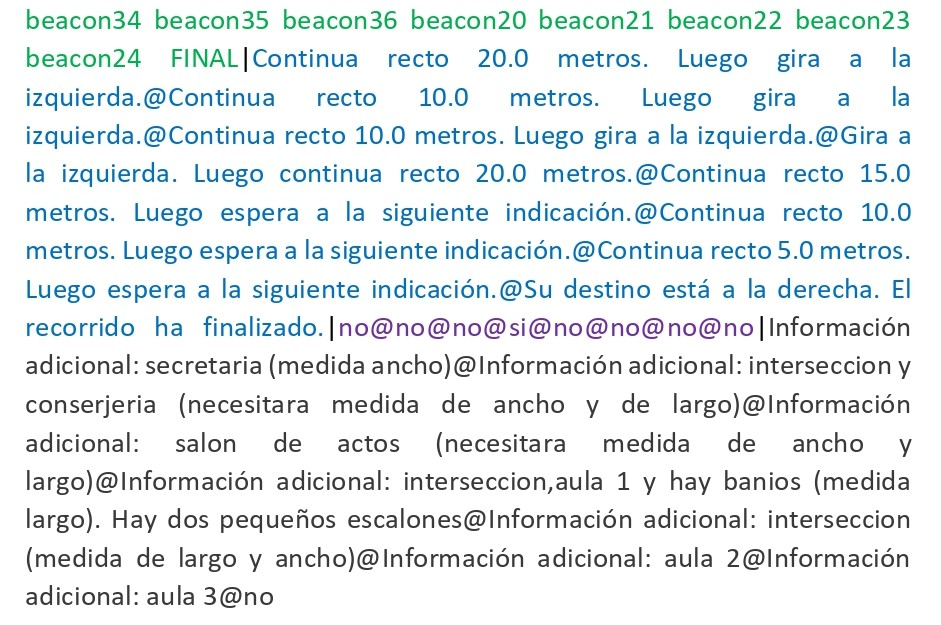
\includegraphics[width=0.9\textwidth]{Imagenes/Capitulo4/ejemploRuta}
	\caption{Ejemplo de la información generada por el servidor para una ruta desde el cuadrante $34$ al $24$.}
	\label{fig:ejemplo_ruta}
\end{figure}


\subsection{Cálculo de la ruta óptima}
\label{sub:rutaOptima}

En esta sección veremos las modificaciones que se han hecho para lograr guiar al usuario por la ruta más conveniente. Como ya hemos visto, el mapeo que hemos visto en la Sección \ref{sec:mapeo} nos proporciona un grafo, en el que los cuadrantes son los nodos y, las conexiones entre ellos, las aristas. Para su representación hemos empleado una matriz de adyacencia y de esta manera, el cálculo de la ruta más corta entre dos cuadrantes se reduce al algoritmo de \textit{Dijkstra}.

Sin embargo, no debemos olvidar que nuestra aplicación tiene un usuario final muy concreto: personas con discapacidad visual. Es por ello que la ruta debe ser lo más sencilla posible, libre de obstáculos y otros elementos que puedan entorpecerles, por lo que en ocasiones la ruta óptima no coincide con la más corta. Para ello, a aquellas conexiones que presenten mayor dificultad para una persona no vidente se les ha asignado un peso mayor, a fin de evitar tomar esa ruta siempre que exista una alternativa. Por ejemplo, la Figura \ref{fig:ruta_optima} ilustra está situación: si quisiéramos ir desde el aula 3 (cuadrante $24$) a la puerta principal (cuadrante $34$), el camino más corto implicaría pasar por delante de los ascensores (ruta roja). Sin embargo, la conexión entre los cuadrantes $31$ y $32$ así como la conexión entre $22$ y $31$ puede resultar tediosa para una persona invidente por varias razones: el tramo compuesto por los cuadrantes $31$, $32$ y $22$ es más estrecho que su camino paralelo por el \textit{hall}, presenta más giros, normalmente, acumula más gente (es zona de paso por los ascensores, escaleras y zona de salida y entrada de la cafetería) y obliga a pasar por dos pequeños peldaños o una rampa estrecha, algo que se convierte en problemático si, además, vamos acompañados de un perro guía o un bastón. Tras el ajuste de pesos en la matriz de adyacencia, la ruta obtenida es la señalada en verde en la Figura \ref{fig:ruta_optima}. De esta manera hacemos que el paso por el pasillo de los ascensores se limite únicamente al caso en el es estrictamente necesario, cuando se va a hacer un cambio de planta.


\begin{figure}[t]
	\centering
	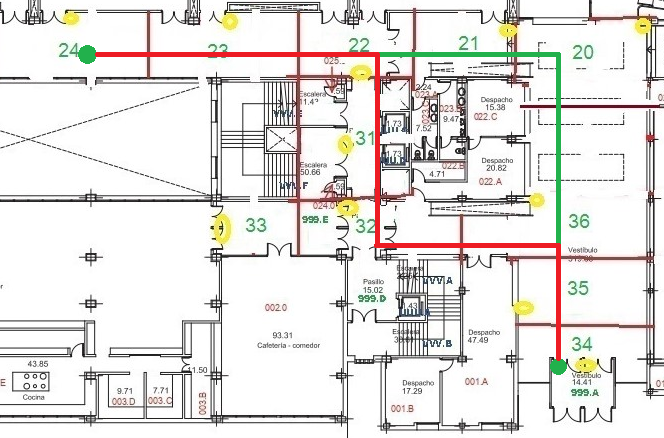
\includegraphics[width=0.8\textwidth]{Imagenes/Capitulo4/mapa_ruta_optima}
	\caption{Ejemplo de ruta óptima entre dos puntos.}
	\label{fig:ruta_optima}
\end{figure}


\subsection{Generación de instrucciones}
\label{sub:genInstruc}

La función que contiene toda la lógica relativa la generación de las instrucciones es \textit{generar}. Esta función es una de las que más modificaciones ha sufrido con respecto a los trabajos predecesores \citep{TFGguia}, pues no solo la hemos adaptado para personas con discapacidad visual sino que también hemos incluido mucha complejidad al añadir cambios de planta y demás casuística que no estaba previamente incluida y que presentamos a continuación:

\begin{itemize}
	\item Se ha añadido a las instrucciones más precisión e información. Cuando el usuario llega al destino, la propia instrucción indica dónde se encuentra. Por ejemplo, ``Su destino está a la derecha'' o a la izquierda o delante del usuario, pues dependiendo de por dónde haya llegado el usuario estará a un lado o a otro. Además, se ha incluido en las instrucciones los metros que el usuario debe recorrer hasta hacer un giro. En la Figura \ref{fig:ejemplo_ruta} podemos ver un ejemplo: a medida que el usuario va recorriendo los cuadrantes la distancia va disminuyendo, lo que hace percibir al usuario que va en el camino correcto. Las instrucciones se van dando en cada cuadrante, sin saltarse hasta ocho cuadrantes como se hacía en \cite{TFGguia}. Esto se ha hecho así porque creemos muy conveniente que el usuario reciba de manera continuada aprobación por parte de la aplicación. En el caso de que la instrucción siguiente corresponde a un giro se invierte el orden y se indica primero este y luego los metros que debe continuar el usuario en la nueva dirección.
	
	
	\item Se han incluido cambios de planta. Esto supone una novedad respecto a \cite{TFGguia}, pues es totalmente nuevo. Ahora los cuadrantes correspondientes a los ascensores están unidos\footnote{El cuadrante $31$ (correspondiente a los ascensores situados detrás de conserjería) está conectado con el $18$ (ascensor correspondiente al anterior en la planta 1) y el $29$ (ascensor más cercano a la puerta trasera de la cafetería) con el $10$ (ascensor correspondiente al anterior en la planta 1).}, permitiendo así que la lista de cuadrantes de la ruta esté formada por cuadrantes de distinta planta. La función \textit{generar} detecta cuando el siguiente cuadrante al que queremos ir no está en la misma planta que el de nuestra posición actual y genera la ruta en consonancia ``Los ascensores están a tu izquierda. Sube a la primera planta.'' o ``El ascensor está delante. Sube a la primera planta.'', por ejemplo. También se tiene en cuenta el caso especial de las zonas de ascensores, pues no son simétricas. Para salir de la zona de los ascensores correspondientes al cuadrante $31$ (los que se sitúan detrás de conserjería) debemos dirigirnos hacia uno de los lados, mientras que para salir de los de la zona de la puerta trasera de la cafetería (cuadrante $29$) debemos caminar hacia adelante para salir de ese vestíbulo. A pesar de que en la Facultad de Informática contamos con ascensores y escaleras, se ha supuesto que la ruta se seguirá por medio de los ascensores ya que de esta manera es más fácil el cambio de planta y, además, estos se encuentran adaptados con botones en \textit{braille}.
	
	\item Otra novedad es que la ruta incluye la posibilidad de informar anticipadamente sobre lo que el usuario se va a encontrar a su paso, como pueden ser pequeños escalones, baños, la cafetería, el despacho de Delegación de Alumnos, etc. Esto es fundamental pues además de dar seguridad al usuario le da la opción de tener una mejor idea global del espacio en el que se encuentra. Para ello lo que se hace es incluir en la ruta la información contenida en el cuadrante siguiente al que se encuentra el usuario, de esta manera conseguimos adelantarnos y avisar al usuario con antelación. Así mismo, la función \textit{generar} da información sobre cuándo el usuario debe hacer un giro para permitir avisar a este de manera especial desde la aplicación del cliente.
	
\end{itemize}


%Comento la figura del diagrama de clases porque quiero ver cómo lo reorganizo
%\begin{figure}[t]
%	\centering
%	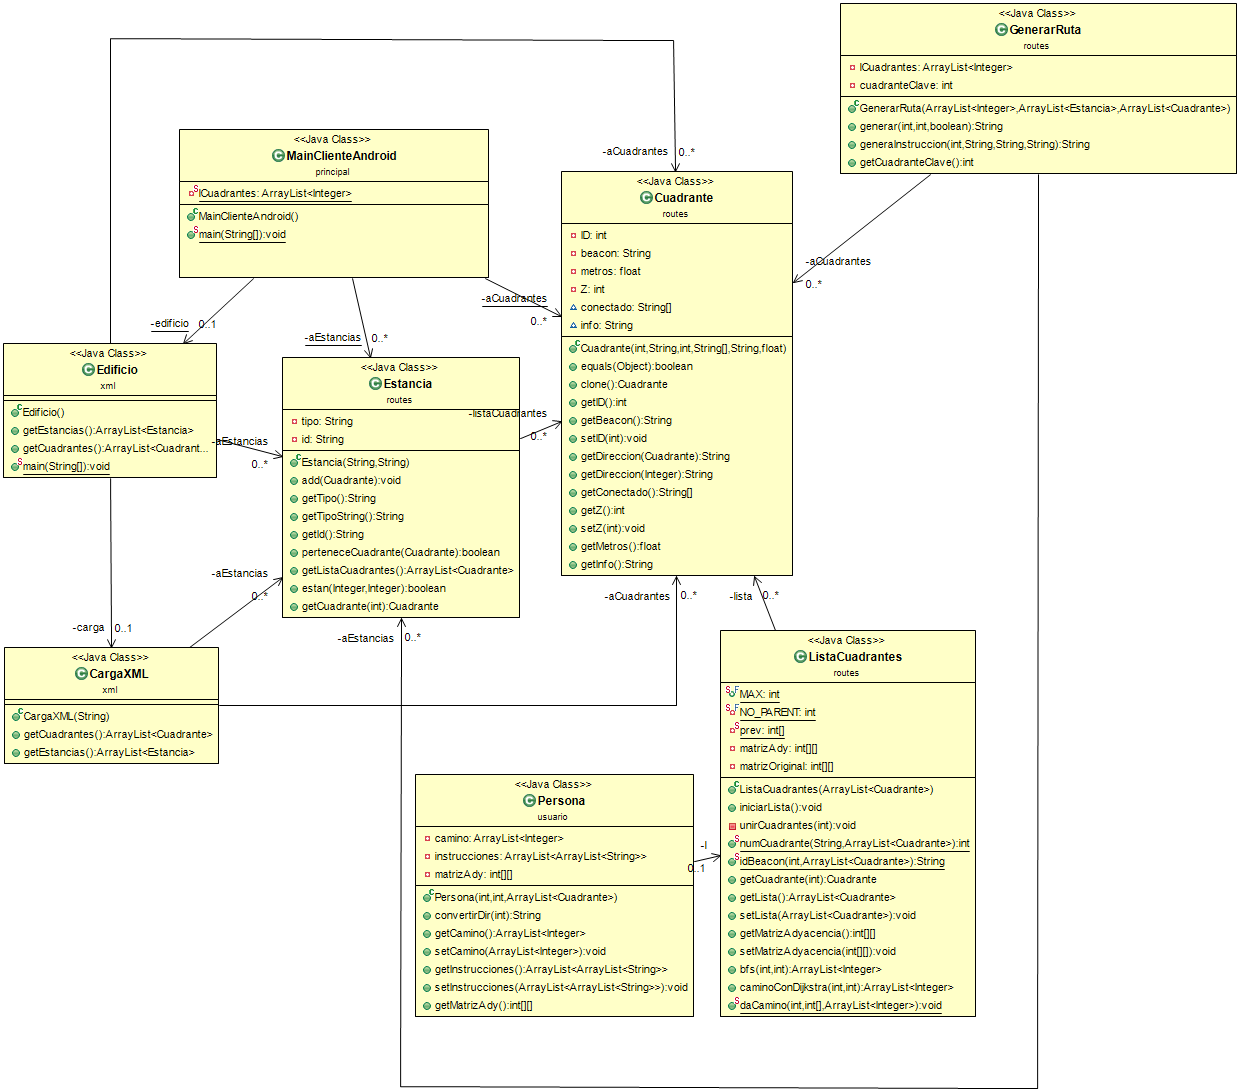
\includegraphics[width=1.1\textwidth]{Imagenes/Capitulo4/diagramServer}
%	\caption{Diagrama de las clases principales del servidor.}
%	\label{fig:diagServ}
%\end{figure}



\section{Cliente}

El cliente de nuestro proyecto está constituido por la aplicación Blind Bit desarrollada para Android. Con esta aplicación podemos conectarnos al servidor e iniciar la ruta al destino deseado desde el punto en el que nos encontremos (siempre que este sea el exterior de las aulas u otras estancias). La aplicación se encarga de darnos, en el momento adecuado, las instrucciones necesarias para llegar al destino y va avisándonos mediante sonidos o vibraciones de diferentes acciones como giros o aprobación de que seguimos en el camino correcto. A continuación presentamos tanto los detalles de diseño de la aplicación como los detalles técnicos de su implementación. 


\subsection{Diseño de la aplicación Blind Bit}

%Aquí hablar de la interfaz y justificar el por qué de las decisiones tomadas (el título de las pantallas, posición y forma de los botones, soniditos y vibraciones, etc) + fotos de la interfaz.

INTRODUCCIÓN (no estoy inspirada)

A continuación describimos las pantallas de nuestra aplicación y los detalles de su diseño:

\begin{itemize}
	\item \textit{Pantalla principal:}
	
	\item \textit{Pantalla de destinos:}
	
	\item \textit{Pantalla de ruta:}
	
	\item \textit{Pantalla modo de uso:}
\end{itemize}

\subsection{Implementación}

En esta sección se exponen los detalles técnicos más relevantes. 

\begin{itemize}
	\item \textit{Conexión con el servidor}: la parte de la clase Cliente
	\item \textit{Seguimiento de la ruta}: la parte de onEddistonUpdate (o como se llame bien)
	\item \textit{Posicionamiento}: El tema de cómo se leen los \textit{beacons}
\end{itemize}
